\documentclass{beamer}
\usefonttheme{professionalfonts}

\usepackage[utf8]{inputenc}
\usepackage{graphicx, xcolor, color}
\usepackage{amsmath, amsthm, amssymb, amsfonts}
\usepackage{bbm}
\usepackage{wasysym}
\usepackage{pifont}
\usepackage{emoji}
\usepackage[absolute, overlay]{textpos}

\usepackage{tikz}
\usepackage{caption}
\captionsetup[figure]{labelformat = empty}
\usepackage{tabularx, booktabs}
\usepackage{multicol}

\usepackage{multirow}
\DeclareMathOperator*{\argmax}{arg\,max}
\DeclareMathOperator*{\argmin}{arg\,min}

\usepackage{color}
\usepackage{minted}
\usepackage{caption}
\captionsetup{font = scriptsize, labelfont = scriptsize}
\setbeamerfont{frametitle}{size=\normalsize}
\setbeamertemplate{section in toc}[ball unnumbered]
% \setbeamertemplate{subsection in toc}[ball unnumbered]

\setbeamertemplate{itemize items}[circle]
\setbeamercolor{itemize item}{fg=black}

\definecolor{light_red}{RGB}{209,105,81}
\definecolor{fair_red}{RGB}{237,27,47}
\definecolor{light_green}{RGB}{58,181,75}
\definecolor{thick_blue}{RGB}{5,43,108}
\definecolor{fair_blue}{RGB}{0,112,192}
\definecolor{light_blue}{RGB}{0,153,228}
\definecolor{light_brown}{RGB}{132, 60, 11}
\usepackage{hyperref}
\hypersetup{
    colorlinks=true,
    linkcolor=blue,
    urlcolor=gray
    }
\setbeamercolor{block title}{fg = black, bg = light_blue!40}
\setbeamercolor{block body}{fg = black, bg = white}
\setbeamertemplate{blocks}[rounded][shadow]
\setbeamercolor{block title example}{fg = black, bg = orange!40}
\setbeamercolor{block body example}{fg = black, bg = white}

\setbeamercolor{block title alerted}{fg = black, bg = light_red!40}
\setbeamercolor{section number projected}{bg=gray}
\setbeamercolor{section number projected}{bg=gray}
\setbeamercolor{subsection number projected}{bg=gray}
\hypersetup{colorlinks=false}

\setbeamertemplate{frametitle}[default][center]
\setbeamertemplate{navigation symbols}{}
\setbeamerfont{footline}{series=\bfseries}
\setbeamertemplate{footline}[frame number]{}

\usefonttheme{professionalfonts}
\usepackage{tikz}
\newcommand{\topline}{
  \tikz[remember picture, overlay] {
    \draw[gray, thick] ([xshift = 1cm, yshift = -1cm]current page.north west)
             -- ([xshift = -1cm, yshift = -1cm, xshift = \paperwidth]current page.north west);}}

\setbeamertemplate{frametitle}[default][center]
\setbeamertemplate{navigation symbols}{}
\setbeamerfont{footline}{series = \bfseries}
\setbeamertemplate{footline}[page number]

\begin{document}

\begin{frame}[plain]

\begin{tikzpicture}[remember picture, overlay]
    \node[xshift=2.7cm,yshift=-1.1cm] at (current page.north west) {
\includegraphics[height = 2.25cm]{graphics/Polytechnique_signature-RGB-gauche_FR.png}};
\end{tikzpicture}

\begin{tikzpicture}[remember picture, overlay]
    \node[xshift=10.5cm,yshift=-1.1cm] at (current page.north west) {
\includegraphics[height = 1.25cm]{graphics/ivado_logo.jpg}};
\end{tikzpicture}

{\color{white}title}

\vspace{3em}

\begin{center}
{\color{black!80}\large\textbf{Low-Rank Matrix and Tensor Factorization}

\vspace{0.2em}

\textbf{for Speed Field Reconstruction}}

\small

\vspace{1.2em}

\textbf{Xinyu Chen}

\vspace{0.4em}

{March 9, 2023}

\vspace{0.5em}

\begin{columns}
\begin{column}{0.3\textwidth}
\begin{figure}
    \centering
    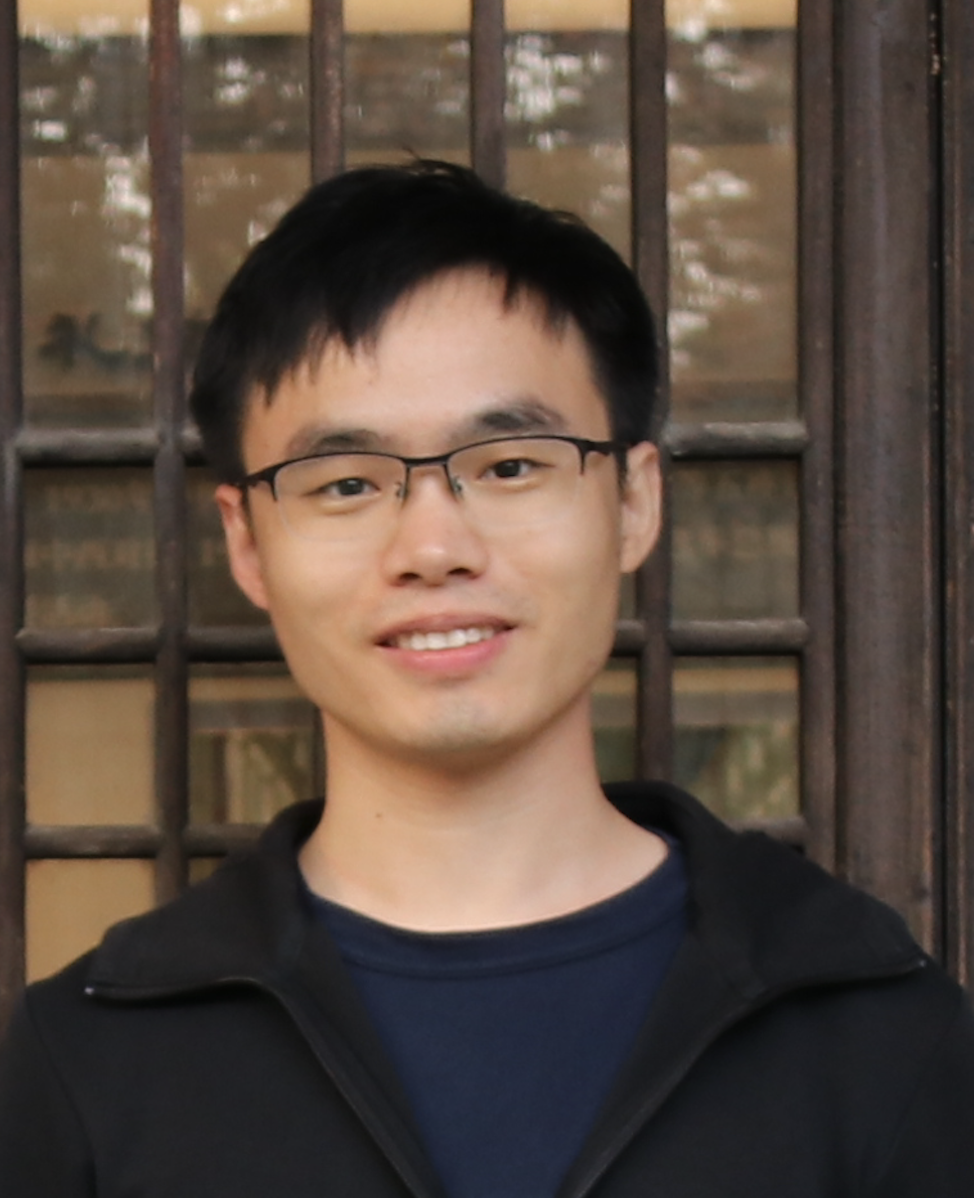
\includegraphics[height = 2.0cm]{graphics/xinyu_chen.png}
    \caption*{\centering\scriptsize \textbf{Ph.D. candidate} \\Xinyu Chen\\ Polytechnique Montr\'eal}
\end{figure}
\end{column}
\hspace{-3em}
\begin{column}{0.3\textwidth}
\begin{figure}
    \centering
    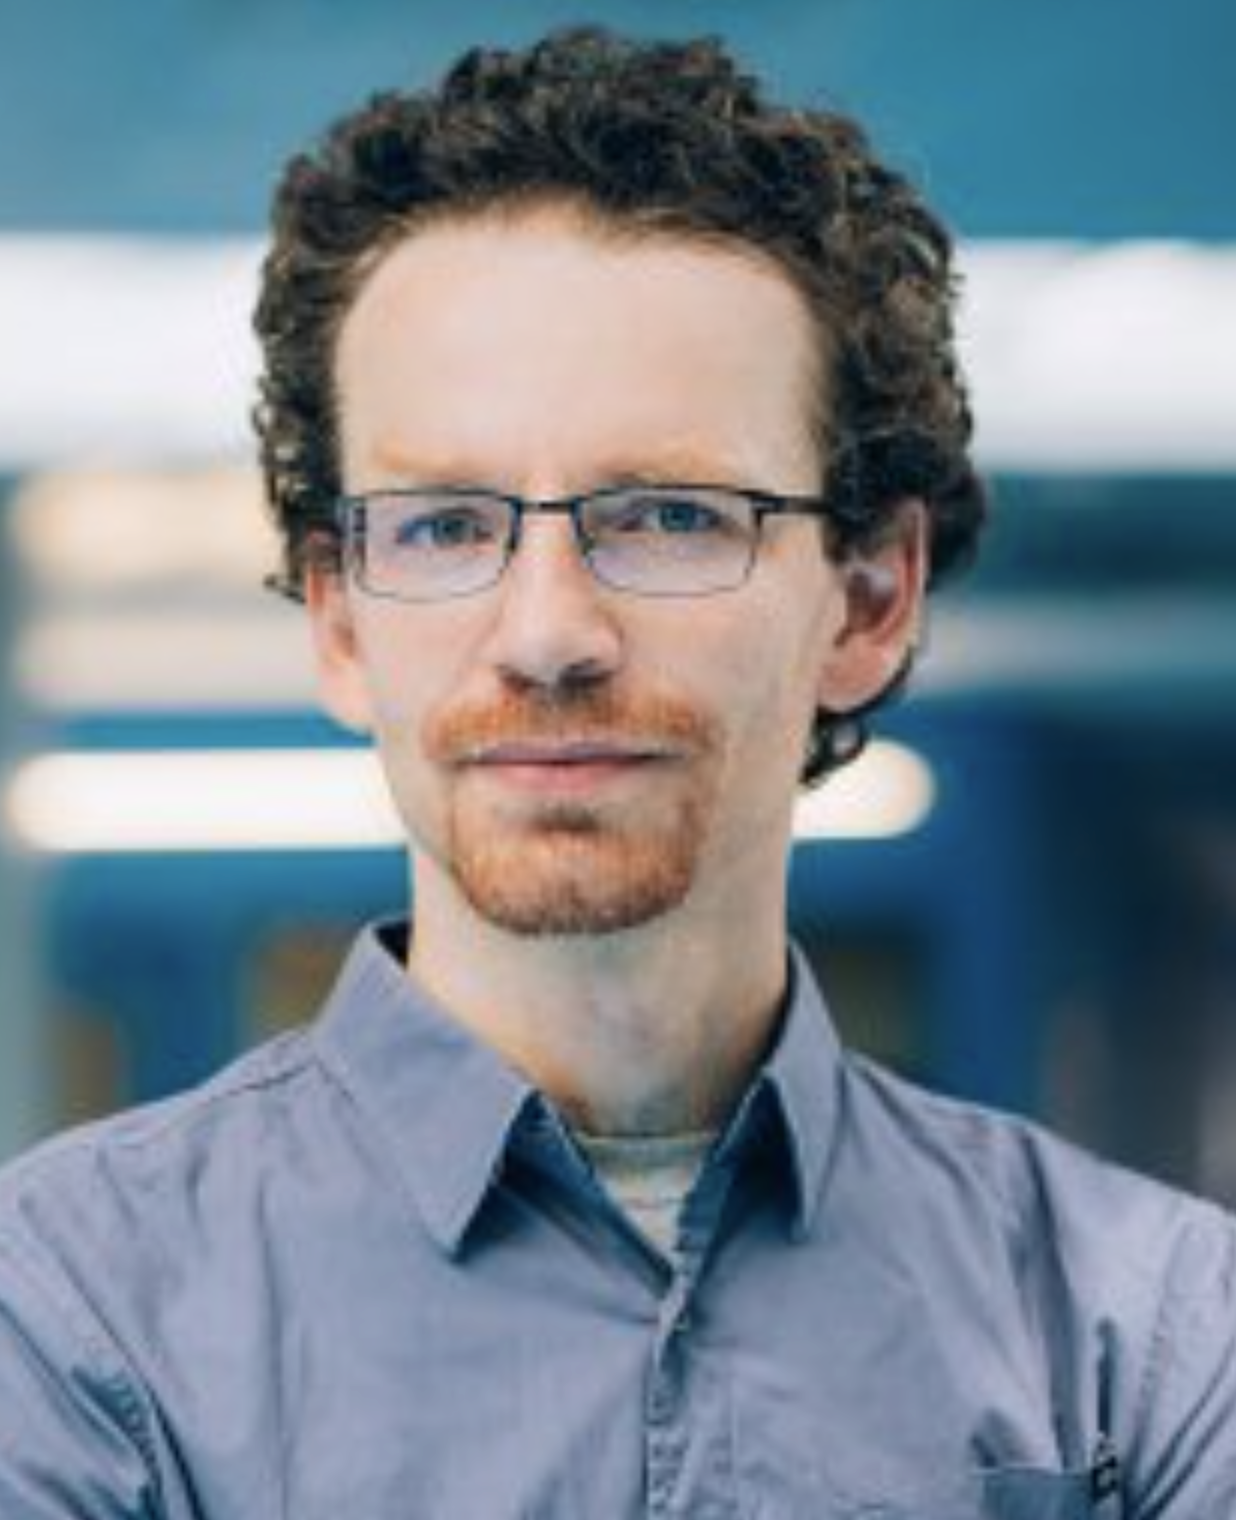
\includegraphics[height = 2cm]{graphics/nicolas_saunier.png}
    \caption*{\centering\scriptsize
    \textbf{Supervisor} \\
    Prof. Nicolas Saunier\\ Polytechnique Montr\'eal}
\end{figure}
\end{column}
\hspace{-3em}
\begin{column}{0.3\textwidth}
\begin{figure}
    \centering
    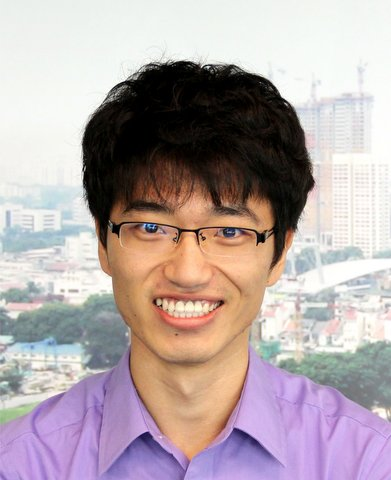
\includegraphics[height = 2cm]{graphics/lijun_sun.jpg}
    \caption*{\centering\scriptsize
    \textbf{Co-supervisor} \\ Prof. Lijun Sun\\ McGill University}
\end{figure}
\end{column}

\end{columns}

\end{center}

\end{frame}

\begin{frame}[plain]
\footnotesize

\begin{itemize}
\item[\color{black}\ding{202}] \textbf{Slides}: {\color{light_blue}\url{https://xinychen.github.io/slides/MF_TF_SFR.pdf}}
\item[\color{black}\ding{203}] \textbf{Jupyter Notebook}: {\color{light_blue}\url{https://github.com/xinychen/transdim/blob/master/toy-examples/MF_TF_SFR.ipynb}}
\end{itemize}

\end{frame}

\begin{frame}[plain]
\frametitle{\color{black}\textbf{Outline}}
\topline
\footnotesize

\tableofcontents

\end{frame}

\section{\color{black}\textbf{Motivation}}

\begin{frame}{\color{black}\textbf{Motivation}}
\topline
\footnotesize

\begin{itemize}
\item Portland highway traffic speed data\footnote{\scriptsize\color{light_blue}\url{https://portal.its.pdx.edu/home}}
\end{itemize}

\begin{center}
\begin{tikzpicture}
\pgfdeclareimage[height = 4cm]{img}{graphics/portland_sensor_stations.png}
\node (img) at (0, 0) {\pgfuseimage{img}};
\node at (0, -2.3) {\color{gray}\scriptsize Highway network \& sensor locations};

\pgfdeclareimage[height = 3.5cm]{img}{graphics/portland_speed_field_I5_NB.png}
\node (img) at (5.5, 0) {\pgfuseimage{img}};
\node at (5.5, -2) {\color{gray}\scriptsize Traffic speed field};
\end{tikzpicture}
\end{center}

\begin{itemize}
\item Speed field $\boldsymbol{Y}\in\mathbb{R}^{N\times T}$ ($N$ locations \& $T$ time steps)
\item Speed field shows strong spatial/temporal dependencies
\end{itemize}

\end{frame}

\begin{frame}{\color{black}\textbf{Motivation}}
\topline
\footnotesize

\begin{center}
\begin{tikzpicture}
\pgfdeclareimage[height = 2.8cm]{img}{graphics/speed_field_80_missing_data.png}
\node (img) at (0, 0) {\pgfuseimage{img}};
\node at (0,-2) {\Large\color{gray}$\Downarrow$};
\node at (-1.5,-1.8) {\scriptsize $200$-by-$500$ matrix};
\node at (-1.5,-2.2) {\scriptsize (NGSIM)};
\node at (2,-1.8) {\scriptsize Reconstruct speed field from};
\node at (2,-2.2) {\scriptsize 20\% sparse trajectories?};
\pgfdeclareimage[height = 2.8cm]{img}{graphics/speed_field_fully_data.png}
\node (img) at (0, -4) {\pgfuseimage{img}};
\end{tikzpicture}
\end{center}

\begin{itemize}
\item How to learn from sparse spatiotemporal data?
\item How to characterize spatial/temporal local dependencies?
\end{itemize}

\end{frame}

\section{\color{black}\textbf{Matrix Factorization}}

\subsection{\color{black}Optimization Problem}

\begin{frame}{\color{black}\textbf{Matrix Factorization}}
\topline
\footnotesize

\begin{itemize}
\item Spatiotemporal data can be reconstructed by low-dimensional latent factors!
\end{itemize}

\begin{center}
\begin{tikzpicture}
\pgfdeclareimage[width=0.9\textwidth]{img}{graphics/matrix_factorization_illustration.pdf}
\node (img) at (0, 0) {\pgfuseimage{img}};

\node [rotate=90] at (-4.9, 0.3) {\color{gray}\scriptsize Spatial locations};
\node at (-3.2, 1.5) {\color{gray}\scriptsize Time steps};
\node at (0, 1.5) {\color{gray}\scriptsize Spatial factors};
\node at (3.2, 1.2) {\color{gray}\scriptsize Temporal factors};

\end{tikzpicture}
\end{center}

\vspace{-1.5em}

\begin{itemize}
\item MF optimization problem
\begin{equation*}
\min_{\boldsymbol{W},\boldsymbol{X}}~\frac{1}{2}\left\|\mathcal{P}_{\Omega}(\boldsymbol{Y}-\boldsymbol{W}^\top\boldsymbol{X})\right\|_{F}^{2}+\frac{\rho}{2}\left(\|\boldsymbol{W}\|_{F}^{2}+\|\boldsymbol{X}\|_{F}^2\right)
\end{equation*}
with factor matrices $\boldsymbol{W}$ and $\boldsymbol{X}$. {\color{gray}\scriptsize($\|\cdot\|_{F}^2$ is the squared Frobenius norm.)}
\begin{itemize}\scriptsize
    \item[\color{black}\circ] Objective function $f(\boldsymbol{W},\boldsymbol{X})$ or $f$;
    \item[\color{black}\circ] Rank $R\in\mathbb{N}^{+}$ ($R<\min\{N,T\}$);
    \item[\color{black}\circ] Orthogonal projection $\mathcal{P}_{\Omega}(\cdot)$.%:\mathbb{R}^{N\times T}\to\mathbb{R}^{N\times T}$
\end{itemize}
\end{itemize}

\end{frame}

\begin{frame}{\color{black}\textbf{Matrix Factorization}}
\topline
\footnotesize

\begin{center}
\begin{tikzpicture}
\pgfdeclareimage[width=0.9\textwidth]{img}{graphics/matrix_factorization_illustration.pdf}
\node (img) at (0, 0) {\pgfuseimage{img}};

\node [rotate=90] at (-4.9, 0.3) {\color{gray}\scriptsize Spatial locations};
\node at (-3.2, 1.5) {\color{gray}\scriptsize Time steps};
\node at (0, 1.5) {\color{gray}\scriptsize Spatial factors};
\node at (3.2, 1.2) {\color{gray}\scriptsize Temporal factors};

\end{tikzpicture}
\end{center}

\vspace{-1em}

\begin{itemize}
\item MF optimization problem
\end{itemize}
\begin{equation*}
\min_{\boldsymbol{W},\boldsymbol{X}}~\frac{1}{2}\left\|\mathcal{P}_{\Omega}(\boldsymbol{Y}-\boldsymbol{W}^\top\boldsymbol{X})\right\|_{F}^{2}+\frac{\rho}{2}\left(\|\boldsymbol{W}\|_{F}^{2}+\|\boldsymbol{X}\|_{F}^2\right)
\end{equation*}

\begin{itemize}
\item Orthogonal projection $\color{cyan!70!black}\mathcal{P}_{\Omega}:\mathbb{R}^{N\times T}\to\mathbb{R}^{N\times T}$?
\begin{itemize}\scriptsize
\item[\color{black}\circ] Simple example: $\color{cyan!70!black}\boldsymbol{Y}=\begin{bmatrix} 1 & 2 \\ 3 & 4 \\ \end{bmatrix}$ with $\color{cyan!70!black}\Omega=\{(1,1),(2,2)\}$, we have
\begin{equation*}
{\color{cyan!70!black}\mathcal{P}_{\Omega}(\boldsymbol{Y})=\begin{bmatrix}
1 & 0 \\ 0 & 4 \\
\end{bmatrix}}
\quad\quad
\mathcal{P}_{\Omega}^{\perp}(\boldsymbol{Y})=\begin{bmatrix}
0 & 2 \\ 3 & 0 \\
\end{bmatrix}\quad\text{(On the complement)}
\end{equation*}
\end{itemize}
\item Role of regularization (with $\rho$): avoid overfitting.
\end{itemize}

\end{frame}

\subsection{\color{black}GD vs. SGD vs. ALS}

\begin{frame}{\color{black}\textbf{Matrix Factorization}}
\topline
\footnotesize

\begin{itemize}
\item MF optimization problem
\end{itemize}

\vspace{-1em}

\begin{equation*}
\min_{\boldsymbol{W},\boldsymbol{X}}~\frac{1}{2}\left\|\mathcal{P}_{\Omega}(\boldsymbol{Y}-\boldsymbol{W}^\top\boldsymbol{X})\right\|_{F}^{2}+\frac{\rho}{2}\left(\|\boldsymbol{W}\|_{F}^{2}+\|\boldsymbol{X}\|_{F}^2\right)
\end{equation*}

\begin{itemize}
\item Partial derivatives
\end{itemize}
\begin{equation*}
\left\{
\begin{aligned}
\frac{\partial f}{\partial\boldsymbol{W}}
&=-\boldsymbol{X}\mathcal{P}_{\Omega}^\top(\boldsymbol{Y}-\boldsymbol{W}^\top\boldsymbol{X})+\rho\boldsymbol{W} \\
\frac{\partial f}{\partial\boldsymbol{X}}
&=-\boldsymbol{W}\mathcal{P}_{\Omega}(\boldsymbol{Y}-\boldsymbol{W}^\top\boldsymbol{X})+\rho\boldsymbol{X} \\
\end{aligned}\right.
\end{equation*}

\begin{itemize}
\item Gradient descent (\textbf{GD}) vs. Steepest gradient descent (\textbf{SGD})
\end{itemize}
\begin{equation*}
\left\{
\begin{aligned}
\boldsymbol{W}:&=\boldsymbol{W}-\alpha\frac{\partial f}{\partial\boldsymbol{W}} \\
\boldsymbol{X}:&=\boldsymbol{X}-\alpha\frac{\partial f}{\partial\boldsymbol{X}} \\
\end{aligned}\right.
\quad\text{vs.}\quad
\left\{
\begin{aligned}
\alpha:=&{\displaystyle\argmin_{\alpha}}~f(\boldsymbol{W}-\alpha \frac{\partial f}{\partial\boldsymbol{W}},\boldsymbol{X}) \\
\boldsymbol{W}:=&\boldsymbol{W}-\alpha \frac{\partial f}{\partial\boldsymbol{W}} \\
\beta:=&{\displaystyle\argmin_{\beta}}~f(\boldsymbol{W},\boldsymbol{X}-\beta \frac{\partial f}{\partial\boldsymbol{X}}) \\
\boldsymbol{X}:=&\boldsymbol{X}-\beta \frac{\partial f}{\partial\boldsymbol{X}} \\
\end{aligned}\right.
\end{equation*}

\begin{itemize}\scriptsize
\item \textbf{Fixed} step size $\alpha$ (\textbf{GD}) vs. \textbf{optimal} step sizes $\{\alpha,\beta\}$ (\textbf{SGD})
\end{itemize}

\end{frame}

\begin{frame}{\color{black}\textbf{Matrix Factorization}}
\topline
\footnotesize

\begin{itemize}
\item MF optimization problem
\end{itemize}

\vspace{-1em}

\begin{equation*}
\min_{\boldsymbol{W},\boldsymbol{X}}~\frac{1}{2}\left\|\mathcal{P}_{\Omega}(\boldsymbol{Y}-\boldsymbol{W}^\top\boldsymbol{X})\right\|_{F}^{2}+\frac{\rho}{2}\left(\|\boldsymbol{W}\|_{F}^{2}+\|\boldsymbol{X}\|_{F}^2\right)
\end{equation*}

\begin{itemize}
\item Partial derivatives
\end{itemize}
\begin{equation*}
\left\{
\begin{aligned}
\frac{\partial f}{\partial\boldsymbol{W}}
&=-\boldsymbol{X}\mathcal{P}_{\Omega}^\top(\boldsymbol{Y}-\boldsymbol{W}^\top\boldsymbol{X})+\rho\boldsymbol{W} \\
\frac{\partial f}{\partial\boldsymbol{X}}
&=-\boldsymbol{W}\mathcal{P}_{\Omega}(\boldsymbol{Y}-\boldsymbol{W}^\top\boldsymbol{X})+\rho\boldsymbol{X} \\
\end{aligned}\right.
\end{equation*}

\begin{itemize}
\item Alternating least squares (\textbf{ALS})
\end{itemize}
\begin{equation*}
\left\{
\begin{aligned}
\frac{\partial f}{\partial\boldsymbol{W}}&=\boldsymbol{0} \\
\frac{\partial f}{\partial\boldsymbol{X}}&=\boldsymbol{0} \\
\end{aligned}\right.
\Longrightarrow
\left\{
\begin{aligned}
\boldsymbol{w}_i&:=\Bigl(\sum_{t:(i,t)\in\Omega}\boldsymbol{x}_t\boldsymbol{x}_t^\top+\rho\boldsymbol{I}_{R}\Bigr)^{-1}\sum_{t:(i,t)\in\Omega}\boldsymbol{x}_ty_{i,t} \\
\boldsymbol{x}_t&:=\Bigl(\sum_{i:(i,t)\in\Omega}\boldsymbol{w}_i\boldsymbol{w}_i^\top+\rho\boldsymbol{I}_{R}\Bigr)^{-1}\sum_{i:(i,t)\in\Omega}\boldsymbol{w}_iy_{i,t} \\
\end{aligned}\right.
\end{equation*}

\begin{itemize}
\item Latent factors
\begin{itemize}\scriptsize
    \item[\color{black}\circ] $\boldsymbol{w}_{i}\in\mathbb{R}^{R},\,i=1,2,\ldots,N$ are the columns of $\boldsymbol{W}$;
    \item[\color{black}\circ] $\boldsymbol{x}_{t}\in\mathbb{R}^{R},\,t=1,2,\ldots,T$ are the columns of $\boldsymbol{X}$.
\end{itemize}
\end{itemize}

\end{frame}

\begin{frame}{\color{black}\textbf{Matrix Factorization}}
\topline
\footnotesize

\textbf{Speed field reconstruction}
\begin{itemize}
\item Objective function $f$ vs. iteration
\begin{itemize}\scriptsize
    \item[\color{black}\circ] Set rank $R=10$, weight parameter $\rho=10$;
    \item[\color{black}\circ] Set GD step size $\alpha=10^{-4}$.
\end{itemize}
\end{itemize}

\begin{center}
\begin{tikzpicture}
\pgfdeclareimage[height = 3.5cm]{img}{graphics/MF_convergence_over_gd_and_als_within_1000iter.pdf}
\node (img) at (0, 0) {\pgfuseimage{img}};
\pgfdeclareimage[height = 3.5cm]{img}{graphics/MF_convergence_over_gd_and_als_within_100iter.pdf}
\node (img) at (5, 0) {\pgfuseimage{img}};
\end{tikzpicture}
\end{center}

\end{frame}

\begin{frame}[plain]
\footnotesize

\begin{center}
\begin{tikzpicture}
\pgfdeclareimage[height = 2.2cm]{img}{graphics/speed_field_80_missing_data.png}
\node (img) at (0, 0) {\pgfuseimage{img}};
\node at (0,-1.3) {\scriptsize Sparse speed field};
\pgfdeclareimage[height = 2.2cm]{img}{graphics/speed_field_MF_gd_rec.png}
\node (img) at (5.8, 0) {\pgfuseimage{img}};
\node at (5.8,-1.3) {\scriptsize MF with GD};
\pgfdeclareimage[height = 2.2cm]{img}{graphics/speed_field_MF_sgd_rec.png}
\node (img) at (0, 0-3) {\pgfuseimage{img}};
\node at (0,-1.3-3) {\scriptsize MF with SGD};
\pgfdeclareimage[height = 2.2cm]{img}{graphics/speed_field_MF_als_rec.png}
\node (img) at (5.8, 0-3) {\pgfuseimage{img}};
\node at (5.8,-1.3-3) {\scriptsize MF with ALS};
\end{tikzpicture}
\end{center}

\begin{itemize}
\item Reconstruction errors
\end{itemize}

\scriptsize
\begin{equation*}
\text{MAPE}=\begin{cases}
50.66\%\quad\text{(GD)} \\ 45.13\% \quad\text{(SGD)} \\ 45.84\% \quad\text{(ALS)}
\end{cases}\quad\quad
\text{RMSE}=\begin{cases}
2.33\quad\text{(GD)} \\ 2.79\quad\text{(SGD)} \\ 2.80\quad\text{(ALS)}
\end{cases}\text{(mph)}
\end{equation*}

\end{frame}

\begin{frame}{\color{black}\textbf{Matrix Factorization}}
\topline
\footnotesize

\textbf{Seattle freeway traffic speed dataset} {\scriptsize\color{gray}(randomly mask 60\% entries)}
\begin{itemize}
\item Dataset: 323 loop detectors \& 8,064 time steps (288 per day)
\item Objective function $f$ vs. iteration
\begin{itemize}\scriptsize
    \item[\color{black}\circ] Set rank $R=10$, weight parameter $\rho=10^2$;
    \item[\color{black}\circ] Set GD step size $\alpha=2\times10^{-5}$.
\end{itemize}
\end{itemize}

\begin{center}
\begin{tikzpicture}
\pgfdeclareimage[height = 3.5cm]{img}{graphics/MF_convergence_over_gd_and_als_within_1000iter_Seattle.pdf}
\node (img) at (0, 0) {\pgfuseimage{img}};
\pgfdeclareimage[height = 3.5cm]{img}{graphics/MF_convergence_over_gd_and_als_within_200iter_Seattle.pdf}
\node (img) at (5, 0) {\pgfuseimage{img}};
\end{tikzpicture}
\end{center}

\vspace{-1em}

\begin{itemize}
\item[\color{black}\circ] Reconstruction errors
\end{itemize}

\scriptsize
\begin{equation*}
\text{MAPE}=\begin{cases}
9.14\%\quad\text{(GD)} \\ 9.12\% \quad\text{(SGD)} \\ 9.13\% \quad\text{(ALS)}
\end{cases}\quad\quad
\text{RMSE}=\begin{cases}
5.24\quad\text{(GD)} \\ 5.24\quad\text{(SGD)} \\ 5.24\quad\text{(ALS)}
\end{cases}\text{(mph)}
\end{equation*}

\end{frame}

\section{\color{black}\textbf{Smoothing Matrix Factorization}}

\subsection{\color{black}Spatial/Temporal Smoothing}

\begin{frame}{\color{black}\textbf{Smoothing Matrix Factorization}}
\topline
\footnotesize

\begin{itemize}
\item Spatial/temporal local dependencies are also important!
\end{itemize}

\begin{center}
\begin{tikzpicture}
\pgfdeclareimage[width=0.9\textwidth]{img}{graphics/smoothing_matrix_factorization_illustration.pdf}
\node (img) at (0, 0) {\pgfuseimage{img}};

\node [rotate=90] at (-4.9, 0.3) {\color{gray}\scriptsize Spatial locations};
\node at (-3.2, 1.5) {\color{gray}\scriptsize Time steps};
\node at (0, 1.5) {\color{gray}\scriptsize Spatial factors};
\node at (3.2, 1.5) {\color{gray}\scriptsize Temporal factors};

\end{tikzpicture}
\end{center}

\vspace{-1em}

\begin{itemize}
\item Formulate spatial/temporal dependencies
\end{itemize}

\begin{equation*}
\begin{aligned}
\boldsymbol{W}\boldsymbol{\Psi}_1^\top=
&\begin{bmatrix}
\mid & & \mid \\ \color{orange!70!black}\boldsymbol{w}_2-\boldsymbol{w}_1 & \cdots & \color{orange!70!black}\boldsymbol{w}_N-\boldsymbol{w}_{N-1} \\ \mid & & \mid \\
\end{bmatrix} \\
\boldsymbol{X}\boldsymbol{\Psi}_2^\top=
&\begin{bmatrix}
\mid & & \mid \\ \color{red!80!black}\boldsymbol{x}_2-\boldsymbol{x}_1 & \cdots & \color{red!80!black}\boldsymbol{x}_T-\boldsymbol{x}_{T-1} \\ \mid & & \mid \\
\end{bmatrix}
\end{aligned}
\end{equation*}

\end{frame}

\subsection{\color{black}Alternating Minimization}

\begin{frame}{\color{black}\textbf{Smoothing Matrix Factorization}}
\topline
\footnotesize

\begin{itemize}
\item Formulate spatial/temporal dependencies
\end{itemize}

\vspace{-1em}

\begin{equation*}
\boldsymbol{\Psi}=\begin{bmatrix}
-1 & 1 & 0 & \cdots & 0 & 0 \\
0 & -1 & 1 & \cdots & 0 & 0 \\
0 & 0 & -1 & \cdots & 0 & 0 \\
\vdots & \vdots & \vdots & \ddots & \vdots & \vdots \\
0 & 0 & 0 & \cdots & -1 & 1 \\
\end{bmatrix}
\Longrightarrow
\left\{
\begin{aligned}
&\|\boldsymbol{W}\boldsymbol{\Psi}_1^\top\|_{F}^{2}\quad\text{with $\boldsymbol{\Psi}_1\in\mathbb{R}^{(N-1)\times N}$} \\
&\|\boldsymbol{X}\boldsymbol{\Psi}_2^\top\|_{F}^{2}\quad\text{with $\boldsymbol{\Psi}_2\in\mathbb{R}^{(T-1)\times T}$}
\end{aligned}\right.
\end{equation*}

\begin{itemize}
\item SMF optimization problem
\end{itemize}
\begin{equation*}
\begin{aligned}
\min_{\boldsymbol{W},\boldsymbol{X}}~&\frac{1}{2}\left\|\mathcal{P}_{\Omega}(\boldsymbol{Y}-\boldsymbol{W}^\top\boldsymbol{X})\right\|_{F}^{2}+\frac{\rho}{2}(\|\boldsymbol{W}\|_{F}^{2}+\|\boldsymbol{X}\|_{F}^{2}) \\
&+\frac{\lambda}{2} (\|\boldsymbol{W}\boldsymbol{\Psi}_{1}^\top\|_{F}^{2}+\|\boldsymbol{X}\boldsymbol{\Psi}_{2}^\top\|_{F}^{2})
\end{aligned}
\end{equation*}

\begin{itemize}
\item \textbf{Alternating minimization}
\end{itemize}

\begin{equation*}
\begin{aligned}
\boldsymbol{W}:=\{\boldsymbol{W}\mid\frac{\partial f}{\partial\boldsymbol{W}}=\boldsymbol{0}\}\quad\quad
\boldsymbol{X}:=\{\boldsymbol{X}\mid\frac{\partial f}{\partial\boldsymbol{X}}=\boldsymbol{0}\}
\end{aligned}
\end{equation*}

\begin{itemize}
\item Solve each matrix equation by the \textbf{conjugate gradient} method.
\end{itemize}

\end{frame}

\begin{frame}{\color{black}\textbf{Smoothing Matrix Factorization}}
\topline
\footnotesize

\begin{itemize}
\item Speed field reconstruction
\begin{itemize}\scriptsize
\item[\color{black}\circ] Set rank $R=10$, weight parameter $\rho=10$.
\item[\color{black}\circ] Recall that the reconstruction errors of MF:
\begin{equation*}
\text{MAPE}=\begin{cases}
50.66\%\quad\text{(GD)} \\ 45.13\% \quad\text{(SGD)} \\ 45.84\% \quad\text{(ALS)}
\end{cases}\quad\quad
\text{RMSE}=\begin{cases}
2.33\quad\text{(GD)} \\ 2.79\quad\text{(SGD)} \\ 2.80\quad\text{(ALS)}
\end{cases}\text{(mph)}
\end{equation*}
\end{itemize}
\end{itemize}

\begin{center}
\begin{tikzpicture}
\pgfdeclareimage[height = 2.2cm]{img}{graphics/speed_field_SMF_rec_lambda_10.png}
\node (img) at (0, 0) {\pgfuseimage{img}};
\node at (0,1.3) {\scriptsize SMF ($\lambda=10$)};
\node at (0,-1.3) {\scriptsize MAPE = \textbf{44.06\%}, RMSE = 2.16mph};
\pgfdeclareimage[height = 2.2cm]{img}{graphics/speed_field_SMF_rec_lambda_100.png}
\node (img) at (5.8, 0) {\pgfuseimage{img}};
\node at (5.8,1.3) {\scriptsize SMF ($\lambda=10^2$)};
\node at (5.8,-1.3) {\scriptsize MAPE = 48.00\%, RMSE = \textbf{1.60mph}};
\end{tikzpicture}
\end{center}

\end{frame}


\section{\color{black}\textbf{Tensor Factorization}}

\subsection{\color{black}Basic Idea}

\begin{frame}{\color{black}\textbf{Tensor Factorization}}
\topline
\footnotesize

\begin{itemize}
\item What is tensor? $\boldsymbol{X}\in\mathbb{R}^{m\times n}$ vs. $\boldsymbol{\mathcal{X}}\in\mathbb{R}^{m\times n\times t}$
\end{itemize}

\begin{center}
\begin{tikzpicture}
\pgfdeclareimage[width=2cm]{img}{graphics/matrix_element.pdf}
\node (img) at (0, -0.2) {\pgfuseimage{img}};
\pgfdeclareimage[width=2.5cm]{img}{graphics/tensor_element.pdf}
\node (img) at (3.5, 0) {\pgfuseimage{img}};
\end{tikzpicture}
\end{center}

\vspace{-1em}

\begin{itemize}
\item Tensors are everywhere!
\end{itemize}

\begin{center}
\begin{tikzpicture}
\pgfdeclareimage[height=2cm]{img}{graphics/gaint_panda_rgb.jpg}
\node (img) at (0, -0.2) {\pgfuseimage{img}};
\node at (0, -1.5) {\color{gray}\scriptsize Color image with};
\node at (0, -1.9) {\color{gray}\scriptsize RGB channels};

\pgfdeclareimage[height=2.5cm]{img}{graphics/fluid_flow_heatmap_2_times_4.png}
\node (img) at (5.2, -0.2) {\pgfuseimage{img}};
\node at (5.2, -1.7) {\color{gray}\scriptsize Dynamical system (fluid flow)};
\end{tikzpicture}
\end{center}

\end{frame}

\begin{frame}[plain]

\begin{center}
\resizebox{10.5cm}{!}{
\begin{tikzpicture}

\pgfdeclareimage[height = 3.6cm]{hitchcock}{graphics/Hitchcock.jpg}
\draw (0, 2.3) node {\color{light_red}\textbf{\large{Higher-Order SVD}}};
\node (hitchcock) at (0, -0.4) {\pgfuseimage{hitchcock}};
\draw (0, -2.7) node {\large\textbf{Frank Lauren Hitchcock}};

\node [circle, line width = 1mm, draw = light_blue, fill = white, minimum size = 0.4cm] (node1) at (0, 3.2) {};
\draw (0, 4) node {\Large\textbf{1927}};

\node [circle, line width = 1mm, draw = light_blue, fill = white, minimum size = 0.4cm] (node2) at (5, 3.2) {};
\draw (5, 4) node {\Large\textbf{1960s}};
\draw (5, 2.3) node {\color{light_red}\textbf{\large{Tucker Decomposition}}};
\draw (5, 1.1) node {\large\textbf{Ledyard R. Tucker}};

\path [line width = 1mm, draw = light_blue, -] (node1) edge (node2);

\node [circle, line width = 1mm, draw = light_blue, fill = white, minimum size = 0.4cm] (node3) at (10, 3.2) {};
\draw (10, 4) node {\Large\textbf{1970}};
\draw (10, 2.3) node {\color{light_red}\textbf{\large{CP Decomposition}}};
\draw (10, 1.1) node {\large\textbf{J. Douglas Carroll}};
\draw (10, 0.5) node {\large\textbf{Jih-Jie Chang}};
\draw (10, -0.1) node {\large\textbf{Richard A. Harshman}};

\draw [line width = 1mm, draw = light_blue]  (5.2, 3.2) -- (7.5, 3.2) -- (7.6, 3.5) -- (7.8, 2.9) -- (7.9, 3.2) -- (9.8, 3.2);

\pgfdeclareimage[height = 3.6cm]{Kolda}{graphics/Kolda.jpg}
\node (Kolda) at (15, -0.4) {\pgfuseimage{Kolda}};
\node [circle, line width = 1mm, draw = light_blue, fill = white, minimum size = 0.4cm] (node4) at (15, 3.2) {};
\draw (15, 4) node {\Large\textbf{2009}};
\draw (15, 2.5) node {\color{light_red}\textbf{\large{Tensor Decompositions}}};
\draw (15, 2.0) node {\color{light_red}\textbf{\large{and Applications}}};
\draw (15, -2.7) node {\large\textbf{Tamara G. Kolda}};

\draw [line width = 1mm, draw = light_blue]  (5.2 + 5, 3.2) -- (7.5 + 5, 3.2) -- (7.6 + 5, 3.5) -- (7.8 + 5, 2.9) -- (7.9 + 5, 3.2) -- (9.8 + 5, 3.2);

\pgfdeclareimage[height = 3.6cm]{Oseledets}{graphics/Oseledets.jpg}
\node (Oseledets) at (20, -0.4) {\pgfuseimage{Oseledets}};
\node [circle, line width = 1mm, draw = light_green, fill = white, minimum size = 0.4cm] (node5) at (20, 3.2) {};
\draw (20, 4) node {\Large\textbf{2011}};
\draw (20, 2.5) node {\color{light_red}\textbf{\large{Tensor-Train}}};
\draw (20, 2) node {\color{light_red}\textbf{\large{Decomposition}}};
\draw (20, -2.7) node {\large\textbf{Ivan Oseledets}};

\draw [line width = 1mm, draw = light_blue]  (5.2 + 10, 3.2) -- (7.5 + 10, 3.2) -- (7.6 + 10, 3.5) -- (7.8 + 10, 2.9) -- (7.9 + 10, 3.2) -- (9.8 + 10, 3.2);

\draw [line width = 1mm, draw = light_green]  (5.2 + 15, 3.2) -- (6.5 + 15, 3.2) -- (6.6 + 15, 3.5) -- (6.8 + 15, 2.9) -- (6.9 + 15, 3.2) -- (7.8 + 15, 3.2);

\end{tikzpicture}
}
\end{center}

\end{frame}

\subsection{\color{black}CP Tensor Factorization}

\begin{frame}{\color{black}\textbf{CP Tensor Factorization}}
\topline
\footnotesize

\begin{itemize}
\item Factorize $\boldsymbol{\mathcal{Y}}$ into the combination of three rank-$R$ factor matrices (i.e., low-dimensional latent factors).
\end{itemize}

\begin{center}
    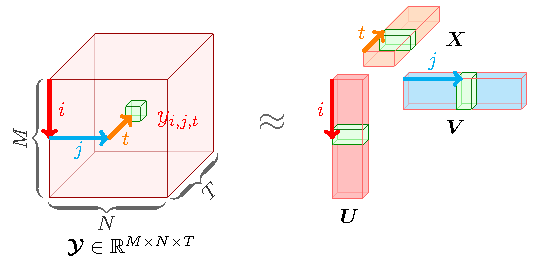
\includegraphics[width=0.6\textwidth]{graphics/third_orderr_CP_factorization_simple_notation.pdf}
\end{center}

\begin{itemize}
\item Understanding CP factorization\footnote{\scriptsize CANDECOMP/PARAFAC (CP) decomposition.}$^,$\footnote{\scriptsize The symbol $\otimes$ denotes the outer product.}:
\begin{equation*}
\left\{
\begin{aligned}
&y_{i,j,t}\approx\sum_{r=1}^{R}u_{i,r}v_{j,r}x_{t,r}
\quad\quad\text{(sum of latent factors)} \\
&\boldsymbol{\mathcal{Y}}\approx\sum_{r=1}^{R}\boldsymbol{u}_{r}\otimes\boldsymbol{v}_{r}\otimes\boldsymbol{x}_{r}
\quad\quad\text{(sum of rank-one tensors)}
\end{aligned}\right.
\end{equation*}
\end{itemize}

\end{frame}

\subsection{\color{black}Hankel Tensor and Its Factorization}

\begin{frame}{\color{black}\textbf{Hankel Tensor and Its Factorization}}
\topline
\footnotesize

\begin{itemize}
\item Hankel matrix
\begin{itemize}\scriptsize
\item[\color{black}\circ] Given $\boldsymbol{y}=(1,2,3,4,5)^\top$ and window length $\tau=2$, we have
\begin{equation*}
\mathcal{H}_{\tau}(\boldsymbol{y})=\begin{bmatrix}
1 & 2 \\ 2 & 3 \\ 3 & 4 \\ 4 & 5 \\
\end{bmatrix}\in\mathbb{R}^{4\times 2}
\end{equation*}

\item[\color{black}\circ] On time series $\boldsymbol{y}=(y_1,y_2,\ldots,y_5)^\top$ with $\tau=2$:
\begin{equation*}
\begin{aligned}
&\mathcal{H}_{\tau}(\boldsymbol{y})=\begin{bmatrix}
y_1 & y_2 \\ y_2 & y_3 \\ y_3 & y_4 \\ y_4 & y_5 \\
\end{bmatrix}\approx\begin{bmatrix}
{\color{cyan!70!black}v_1} \\ 
{\color{cyan!70!black}v_2} \\ {\color{cyan!70!black}v_3} \\ {\color{cyan!70!black}v_4} \\
\end{bmatrix}\otimes\begin{bmatrix}
{\color{orange!70!black}x_1} \\ 
{\color{orange!70!black}x_2} \\
\end{bmatrix} \\
\Longrightarrow\quad\hat{\boldsymbol{y}}=\begin{bmatrix}
\hat{y}_1 \\
\hat{y}_2 \\
\hat{y}_3 \\
\hat{y}_4 \\
\hat{y}_5 \\
\end{bmatrix}=&\mathcal{H}_{\tau}^{-1}\left(\begin{bmatrix}
v_1x_1 & v_1x_2 \\
v_2x_1 & v_2x_2 \\
v_3x_1 & v_3x_2 \\
v_4x_1 & v_4x_2 \\
\end{bmatrix}\right)=\begin{bmatrix}
{\color{cyan!70!black}v_1}{\color{orange!70!black}x_1} \\ ({\color{cyan!70!black}v_1}{\color{orange!70!black}x_2}+{\color{cyan!70!black}v_2}{\color{orange!70!black}x_1})/2 \\ ({\color{cyan!70!black}v_2}{\color{orange!70!black}x_2}+{\color{cyan!70!black}v_3}{\color{orange!70!black}x_1})/2 \\ ({\color{cyan!70!black}v_3}{\color{orange!70!black}x_2}+{\color{cyan!70!black}v_4}{\color{orange!70!black}x_1})/2 \\ {\color{cyan!70!black}v_4}{\color{orange!70!black}x_2} \\
\end{bmatrix}
\end{aligned}
\end{equation*}
\item[\color{black}\circ] Automatic temporal modeling.
\end{itemize}
\end{itemize}

\end{frame}

\begin{frame}{\color{black}\textbf{Hankel Tensor and Its Factorization}}
\topline
\footnotesize

\begin{itemize}
\item (Hankelization) Hankel tensor $\mathcal{H}_{\tau}(\boldsymbol{Y})$
\begin{itemize}\scriptsize
    \item[\color{black}\circ] Tensor size: $N\times (T-\tau+1)\times \tau$;
    \item[\color{black}\circ] Slices: $\boldsymbol{Y}_{k}=\begin{bmatrix}
        \mid & \mid & & \mid \\
        \color{orange!70!black}\boldsymbol{y}_{k} & \color{orange!70!black}\boldsymbol{y}_{k+1} & \cdots & \color{orange!70!black}\boldsymbol{y}_{T-\tau+k} \\
        \mid & \mid & & \mid \\
    \end{bmatrix},\, k=1,2,\ldots,\tau$;
    \item[\color{black}\circ] Slice size: $\color{orange!70!black}N\times(T-\tau+1)$.
\end{itemize}
\end{itemize}

\begin{center}
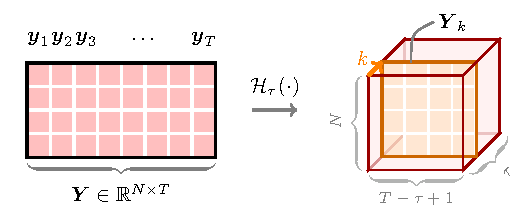
\includegraphics[scale=0.8]{graphics/third_order_Hankel_tensor.pdf}
\end{center}

\end{frame}

\begin{frame}{\color{black}\textbf{Hankel Tensor and Its Factorization}}
\topline
\footnotesize

\begin{itemize}
\item HTF optimization problem
\end{itemize}
\begin{equation*}
\begin{aligned}
\min_{\boldsymbol{U},\boldsymbol{V},\boldsymbol{X}}~&\frac{1}{2}\Bigl\|\mathcal{P}_{\tilde{\Omega}}\Bigl(\mathcal{H}_{\tau}(\boldsymbol{Y})-\sum_{r=1}^{R}\boldsymbol{u}_{r}\otimes\boldsymbol{v}_{r}\otimes\boldsymbol{x}_{r}\Bigr)\Bigr\|_{F}^{2} \\
\end{aligned}
\end{equation*}

\begin{itemize}
\item HTF's advantage/disadvantage over MF:
\begin{itemize}\scriptsize
    \item[\color{black}\ding{51}] Automatic temporal modeling\quad\quad\ding{55}\, High memory consumption
\end{itemize}
\end{itemize}

\begin{itemize}
\item Speed field reconstruction
\begin{itemize}\scriptsize
    \item[\color{black}\circ] Set rank $R=10$;
    \item[\color{black}\circ] Recall that SMF: MAPE = 48.00\% \& RMSE = 1.60mph.
\end{itemize}
\end{itemize}

\begin{center}
\begin{tikzpicture}
\pgfdeclareimage[height = 2.2cm]{img}{graphics/speed_field_HTF_rec_tau_10.png}
\node (img) at (0, 0) {\pgfuseimage{img}};
\node at (0,1.3) {\scriptsize HTF ($\tau=10$)};
\node at (0,-1.3) {\scriptsize MAPE = \textbf{41.40\%}, RMSE = \textbf{1.42mph}};
\pgfdeclareimage[height = 2.2cm]{img}{graphics/speed_field_HTF_rec_tau_15.png}
\node (img) at (5.8, 0) {\pgfuseimage{img}};
\node at (5.8,1.3) {\scriptsize HTF ($\tau=15$)};
\node at (5.8,-1.3) {\scriptsize MAPE = 43.97\%, RMSE = \textbf{1.42mph}};
\end{tikzpicture}
\end{center}

\end{frame}

\section{\color{black}\textbf{Discussion}}

\subsection{\color{black}Which Model Is Better?}

\begin{frame}{\color{black}\textbf{Which Model Is Better?}}
\topline
\footnotesize

\begin{center}
\begin{tikzpicture}
\pgfdeclareimage[height = 2.2cm]{img}{graphics/speed_field_80_missing_data.png}
\node (img) at (0, 0) {\pgfuseimage{img}};
\node at (0,-1.3) {\scriptsize Sparse speed field};

\pgfdeclareimage[height = 2.2cm]{img}{graphics/speed_field_MF_als_rec.png}
\node (img) at (5.8, 1) {\pgfuseimage{img}};
\node at (5.8,2.1) {\scriptsize MF (ALS)};

\pgfdeclareimage[height = 2.2cm]{img}{graphics/speed_field_fully_data.png}
\node (img) at (0, 0-3) {\pgfuseimage{img}};
\node at (0,-1.3-3) {\scriptsize Ground truth speed field};

\pgfdeclareimage[height = 2.2cm]{img}{graphics/speed_field_SMF_rec_lambda_100.png}
\node (img) at (5.8, 1.5-3) {\pgfuseimage{img}};
\node at (5.8,2.6-3) {\scriptsize SMF};

\pgfdeclareimage[height = 2.2cm]{img}{graphics/speed_field_HTF_rec_tau_10.png}
\node (img) at (5.8, -1-3) {\pgfuseimage{img}};
\node at (5.8,0.1-3) {\scriptsize HTF};
\end{tikzpicture}
\end{center}


\end{frame}


\begin{frame}{\color{black}\textbf{Which Model Is Better?}}
\topline
\footnotesize

\begin{center}
\begin{tikzpicture}
\pgfdeclareimage[height = 2.2cm]{img}{graphics/speed_field_80_missing_data.png}
\node (img) at (0, 0) {\pgfuseimage{img}};
\node at (0,-1.3) {\scriptsize Sparse speed field};

\pgfdeclareimage[height = 2.2cm]{img}{graphics/speed_field_MF_als_rec.png}
\node (img) at (5.8, 1) {\pgfuseimage{img}};
\node at (5.8,2.1) {\scriptsize MF (ALS)};
\draw [ultra thick, red] (3.8,1.3) rectangle (4.5,1.95);
\draw [ultra thick, blue] (7,0.4) rectangle (7.7,1.95);

\pgfdeclareimage[height = 2.2cm]{img}{graphics/speed_field_fully_data.png}
\node (img) at (0, 0-3) {\pgfuseimage{img}};
\node at (0,-1.3-3) {\scriptsize Ground truth speed field};
\draw [ultra thick, red] (3.8-5.8,1.3-4) rectangle (4.5-5.8,1.95-4);
\draw [ultra thick, blue] (7-5.8,0.4-4) rectangle (7.7-5.8,1.95-4);

\pgfdeclareimage[height = 2.2cm]{img}{graphics/speed_field_SMF_rec_lambda_100.png}
\node (img) at (5.8, 1.5-3) {\pgfuseimage{img}};
\node at (5.8,2.6-3) {\scriptsize SMF};
\draw [ultra thick, red] (3.8,1.8-3) rectangle (4.5,2.45-3);
\draw [ultra thick, blue] (7,0.9-3) rectangle (7.7,2.45-3);

\pgfdeclareimage[height = 2.2cm]{img}{graphics/speed_field_HTF_rec_tau_10.png}
\node (img) at (5.8, -1-3) {\pgfuseimage{img}};
\node at (5.8,0.1-3) {\scriptsize HTF};
\draw [ultra thick, red] (3.8,-0.7-3) rectangle (4.5,-0.05-3);
\draw [ultra thick, blue] (7,-1.6-3) rectangle (7.7,-0.05-3);
\end{tikzpicture}
\end{center}


\end{frame}

\begin{frame}{\color{black}\textbf{Which Model Is Better?}}
\topline
\footnotesize

\begin{itemize}
\item Seattle freeway traffic speed data
\begin{itemize}\scriptsize
\item[\color{black}\circ] Randomly mask 60\% entries;
\item[\color{black}\circ] SMF: set $R=10$, $\rho=10^2$, $\lambda=2\times 10^2$;
\item[\color{black}\circ] HTF: set $\tau=6$, $R=10$;
\item[\color{black}\circ] Reconstruction errors
\begin{equation*}
\text{MAPE}=\begin{cases}
9.13\% &\text{(MF)} \\
9.01\% &\text{(SMF)} \\
\boldsymbol{8.67\%} &\text{(HTF)} \\
\end{cases}\quad\quad
\text{RMSE}=\begin{cases}
5.24 &\text{(MF)} \\
5.14 &\text{(SMF)} \\
\boldsymbol{5.02} &\text{(HTF)} \\
\end{cases}\text{(mph)}
\end{equation*}
\end{itemize}

\end{itemize}

\end{frame}

\begin{frame}{\color{black}\textbf{Which Model Is Better?}}
\topline
\footnotesize

\begin{itemize}
\item Gray image inpainting
\begin{itemize}\scriptsize
\item[\color{black}\circ] Randomly mask 90\% pixels;
\item[\color{black}\circ] MF: set $R=50$, $\rho=10^{-1}$;
\item[\color{black}\circ] SMF: set $R=50$, $\rho=10^{-1}$, $\lambda=10$.
\end{itemize}
\end{itemize}

\vspace{-1em}

\begin{center}
\begin{tikzpicture}
\pgfdeclareimage[height=2.2cm]{img}{graphics/gaint_panda_gray_missing_rate_90.png}
\node (img) at (0, 0) {\pgfuseimage{img}};
\node at (0, -1.4) {\scriptsize Incomplete image};

\pgfdeclareimage[height=2.2cm]{img}{graphics/gaint_panda_gray_recovery_90_mf_rank_50_lmbda_0.png}
\node (img) at (2.8, 0) {\pgfuseimage{img}};
\node at (2.8, -1.4) {\scriptsize MF};

\pgfdeclareimage[height=2.2cm]{img}{graphics/gaint_panda_gray_recovery_90_mf_rank_50_lmbda_10.png}
\node (img) at (5.6, 0) {\pgfuseimage{img}};
\node at (5.6, -1.4) {\scriptsize SMF};

\pgfdeclareimage[height=2.2cm]{img}{graphics/gaint_panda_gray.png}
\node (img) at (8.4, 0) {\pgfuseimage{img}};
\node at (8.4, -1.4) {\scriptsize Ground truth};

\end{tikzpicture}
\end{center}

\end{frame}

\section{\color{black}\textbf{Conclusion}}

\begin{frame}{\color{black}\textbf{Conclusion}}
\topline
\footnotesize

\begin{itemize}
\item How to reconstruct sparse speed field?
\begin{itemize}\scriptsize
    \item[\color{black}\ding{51}] Matrix factorization ({\color{red!80!black}\textbf{MF}}) \quad\ding{51} Tensor factorization ({\color{red!80!black}\textbf{TF}})
\end{itemize}
\item The importance of spatiotemporal modeling in low-rank methods?
\begin{itemize}\scriptsize
\item[\color{black}\circ] Spatial/temporal {\color{red!80!black}\textbf{smoothing}} regularization:
\end{itemize}
\end{itemize}
\scriptsize
\begin{equation*}
\begin{aligned}
\min_{\boldsymbol{W},\boldsymbol{X}}~&\frac{1}{2}\left\|\mathcal{P}_{\Omega}(\boldsymbol{Y}-\boldsymbol{W}^\top\boldsymbol{X})\right\|_{F}^{2}+\frac{\rho}{2}(\|\boldsymbol{W}\|_{F}^{2}+\|\boldsymbol{X}\|_{F}^{2}) \\
&+\color{red!80!black}\frac{\lambda}{2} (\|\boldsymbol{W}\boldsymbol{\Psi}_{1}^\top\|_{F}^{2}+\|\boldsymbol{X}\boldsymbol{\Psi}_{2}^\top\|_{F}^{2})
\end{aligned}
\end{equation*}
\begin{itemize}
\begin{itemize}\scriptsize
\item[\color{black}\circ] Automatic temporal modeling via {\color{red!80!black}\textbf{Hankelization}}:
\end{itemize}
\end{itemize}
\begin{equation*}
\begin{aligned}
\min_{\boldsymbol{U},\boldsymbol{V},\boldsymbol{X}}~&\frac{1}{2}\Bigl\|\mathcal{P}_{\tilde{\Omega}}\Bigl({\color{red!80!black}\mathcal{H}_{\tau}(\boldsymbol{Y})}-\sum_{r=1}^{R}\boldsymbol{u}_{r}\otimes\boldsymbol{v}_{r}\otimes\boldsymbol{x}_{r}\Bigr)\Bigr\|_{F}^{2} \\
\end{aligned}
\end{equation*}

\end{frame}


\begin{frame}[plain]
\begin{tikzpicture}[remember picture, overlay]
    \node[xshift=2.7cm,yshift=-1.1cm] at (current page.north west) {
\includegraphics[height = 2.25cm]{graphics/Polytechnique_signature-RGB-gauche_FR.png}};
\end{tikzpicture}

\begin{tikzpicture}[remember picture, overlay]
    \node[xshift=10.5cm,yshift=-1.1cm] at (current page.north west) {
\includegraphics[height = 1.25cm]{graphics/ivado_logo.jpg}};
\end{tikzpicture}

\vspace{2em}

\begin{center}
\LARGE Thanks for your attention!

\vspace{1em}

\large Any Questions?
\end{center}

\scriptsize

\vspace{1em}

\textbf{About me}:
\begin{itemize}
\item[\emoji{classical-building}] Homepage:~{\color{light_blue}\url{https://xinychen.github.io}}
\item[\emoji{technologist}] GitHub:~{\color{light_blue}\url{https://github.com/xinychen}} {\scriptsize(\textbf{3k+ stars})}
\item[\emoji{writing-hand}] Blog:~{\color{light_blue}\url{https://medium.com/@xinyu.chen}} {\scriptsize(\textbf{60k+ views})}
\item[\emoji{love-letter}] How to reach me:~{\color{light_blue}\url{chenxy346@gmail.com}}
\end{itemize}

\end{frame}

\end{document}
